% Options for packages loaded elsewhere
\PassOptionsToPackage{unicode}{hyperref}
\PassOptionsToPackage{hyphens}{url}
%
\documentclass[
  10pt,
  letterpaper,
  DIV=11,
  numbers=noendperiod,
  twoside]{scrartcl}

\usepackage{amsmath,amssymb}
\usepackage{setspace}
\usepackage{iftex}
\ifPDFTeX
  \usepackage[T1]{fontenc}
  \usepackage[utf8]{inputenc}
  \usepackage{textcomp} % provide euro and other symbols
\else % if luatex or xetex
  \usepackage{unicode-math}
  \defaultfontfeatures{Scale=MatchLowercase}
  \defaultfontfeatures[\rmfamily]{Ligatures=TeX,Scale=1}
\fi
\usepackage{lmodern}
\ifPDFTeX\else  
    % xetex/luatex font selection
  \setmainfont[ItalicFont=EB Garamond Italic,BoldFont=EB Garamond
Bold]{EB Garamond Math}
  \setsansfont[]{Europa-Bold}
  \setmathfont[]{Garamond-Math}
\fi
% Use upquote if available, for straight quotes in verbatim environments
\IfFileExists{upquote.sty}{\usepackage{upquote}}{}
\IfFileExists{microtype.sty}{% use microtype if available
  \usepackage[]{microtype}
  \UseMicrotypeSet[protrusion]{basicmath} % disable protrusion for tt fonts
}{}
\usepackage{xcolor}
\usepackage[left=1in, right=1in, top=0.8in, bottom=0.8in,
paperheight=9.5in, paperwidth=6.5in, includemp=TRUE, marginparwidth=0in,
marginparsep=0in]{geometry}
\setlength{\emergencystretch}{3em} % prevent overfull lines
\setcounter{secnumdepth}{3}
% Make \paragraph and \subparagraph free-standing
\ifx\paragraph\undefined\else
  \let\oldparagraph\paragraph
  \renewcommand{\paragraph}[1]{\oldparagraph{#1}\mbox{}}
\fi
\ifx\subparagraph\undefined\else
  \let\oldsubparagraph\subparagraph
  \renewcommand{\subparagraph}[1]{\oldsubparagraph{#1}\mbox{}}
\fi


\providecommand{\tightlist}{%
  \setlength{\itemsep}{0pt}\setlength{\parskip}{0pt}}\usepackage{longtable,booktabs,array}
\usepackage{calc} % for calculating minipage widths
% Correct order of tables after \paragraph or \subparagraph
\usepackage{etoolbox}
\makeatletter
\patchcmd\longtable{\par}{\if@noskipsec\mbox{}\fi\par}{}{}
\makeatother
% Allow footnotes in longtable head/foot
\IfFileExists{footnotehyper.sty}{\usepackage{footnotehyper}}{\usepackage{footnote}}
\makesavenoteenv{longtable}
\usepackage{graphicx}
\makeatletter
\def\maxwidth{\ifdim\Gin@nat@width>\linewidth\linewidth\else\Gin@nat@width\fi}
\def\maxheight{\ifdim\Gin@nat@height>\textheight\textheight\else\Gin@nat@height\fi}
\makeatother
% Scale images if necessary, so that they will not overflow the page
% margins by default, and it is still possible to overwrite the defaults
% using explicit options in \includegraphics[width, height, ...]{}
\setkeys{Gin}{width=\maxwidth,height=\maxheight,keepaspectratio}
% Set default figure placement to htbp
\makeatletter
\def\fps@figure{htbp}
\makeatother
% definitions for citeproc citations
\NewDocumentCommand\citeproctext{}{}
\NewDocumentCommand\citeproc{mm}{%
  \begingroup\def\citeproctext{#2}\cite{#1}\endgroup}
\makeatletter
 % allow citations to break across lines
 \let\@cite@ofmt\@firstofone
 % avoid brackets around text for \cite:
 \def\@biblabel#1{}
 \def\@cite#1#2{{#1\if@tempswa , #2\fi}}
\makeatother
\newlength{\cslhangindent}
\setlength{\cslhangindent}{1.5em}
\newlength{\csllabelwidth}
\setlength{\csllabelwidth}{3em}
\newenvironment{CSLReferences}[2] % #1 hanging-indent, #2 entry-spacing
 {\begin{list}{}{%
  \setlength{\itemindent}{0pt}
  \setlength{\leftmargin}{0pt}
  \setlength{\parsep}{0pt}
  % turn on hanging indent if param 1 is 1
  \ifodd #1
   \setlength{\leftmargin}{\cslhangindent}
   \setlength{\itemindent}{-1\cslhangindent}
  \fi
  % set entry spacing
  \setlength{\itemsep}{#2\baselineskip}}}
 {\end{list}}
\usepackage{calc}
\newcommand{\CSLBlock}[1]{\hfill\break\parbox[t]{\linewidth}{\strut\ignorespaces#1\strut}}
\newcommand{\CSLLeftMargin}[1]{\parbox[t]{\csllabelwidth}{\strut#1\strut}}
\newcommand{\CSLRightInline}[1]{\parbox[t]{\linewidth - \csllabelwidth}{\strut#1\strut}}
\newcommand{\CSLIndent}[1]{\hspace{\cslhangindent}#1}

\setlength\heavyrulewidth{0ex}
\setlength\lightrulewidth{0ex}
\usepackage[automark]{scrlayer-scrpage}
\clearpairofpagestyles
\cehead{
  Brian Weatherson
  }
\cohead{
  Decision Making with Imprecise Probabilities
  }
\ohead{\bfseries \pagemark}
\cfoot{}
\makeatletter
\newcommand*\NoIndentAfterEnv[1]{%
  \AfterEndEnvironment{#1}{\par\@afterindentfalse\@afterheading}}
\makeatother
\NoIndentAfterEnv{itemize}
\NoIndentAfterEnv{enumerate}
\NoIndentAfterEnv{description}
\NoIndentAfterEnv{quote}
\NoIndentAfterEnv{equation}
\NoIndentAfterEnv{longtable}
\NoIndentAfterEnv{abstract}
\renewenvironment{abstract}
 {\vspace{-1.25cm}
 \quotation\small\noindent\rule{\linewidth}{.5pt}\par\smallskip
 \noindent }
 {\par\noindent\rule{\linewidth}{.5pt}\endquotation}
\KOMAoption{captions}{tableheading}
\makeatletter
\@ifpackageloaded{caption}{}{\usepackage{caption}}
\AtBeginDocument{%
\ifdefined\contentsname
  \renewcommand*\contentsname{Table of contents}
\else
  \newcommand\contentsname{Table of contents}
\fi
\ifdefined\listfigurename
  \renewcommand*\listfigurename{List of Figures}
\else
  \newcommand\listfigurename{List of Figures}
\fi
\ifdefined\listtablename
  \renewcommand*\listtablename{List of Tables}
\else
  \newcommand\listtablename{List of Tables}
\fi
\ifdefined\figurename
  \renewcommand*\figurename{Figure}
\else
  \newcommand\figurename{Figure}
\fi
\ifdefined\tablename
  \renewcommand*\tablename{Table}
\else
  \newcommand\tablename{Table}
\fi
}
\@ifpackageloaded{float}{}{\usepackage{float}}
\floatstyle{ruled}
\@ifundefined{c@chapter}{\newfloat{codelisting}{h}{lop}}{\newfloat{codelisting}{h}{lop}[chapter]}
\floatname{codelisting}{Listing}
\newcommand*\listoflistings{\listof{codelisting}{List of Listings}}
\makeatother
\makeatletter
\makeatother
\makeatletter
\@ifpackageloaded{caption}{}{\usepackage{caption}}
\@ifpackageloaded{subcaption}{}{\usepackage{subcaption}}
\makeatother
\ifLuaTeX
  \usepackage{selnolig}  % disable illegal ligatures
\fi
\usepackage{bookmark}

\IfFileExists{xurl.sty}{\usepackage{xurl}}{} % add URL line breaks if available
\urlstyle{same} % disable monospaced font for URLs
\hypersetup{
  pdftitle={Decision Making with Imprecise Probabilities},
  pdfauthor={Brian Weatherson},
  hidelinks,
  pdfcreator={LaTeX via pandoc}}

\title{Decision Making with Imprecise Probabilities}
\author{Brian Weatherson}
\date{1998}

\begin{document}
\maketitle
\begin{abstract}
Orthodox Bayesian decision theory requires an agent's beliefs
representable by a real-valued function, ideally a probability function.
Many theorists have argued this is too restrictive; it can be perfectly
reasonable to have indeterminate degrees of belief. So doxastic states
are ideally representable by a set of probability functions. One
consequence of this is that the expected value of a gamble will be
imprecise. This paper looks at the attempts to extend Bayesian decision
theory to deal with such cases, and concludes that all proposals
advanced thus far have been incoherent. A more modest, but coherent,
alternative is proposed.
\end{abstract}

\setstretch{1.1}
\section{Introduction}\label{introduction}

Orthodox Bayesian decision theory requires agents' doxastic states to be
represented by a probability function, the so-called `subjective
probabilities', and their desires to be represented by a real-valued
utility function. Once these idealisations are in place, decision theory
becomes relatively straightforward. The best choice is the one with the
highest expected utility according to the probability function. Because
of Newcomb-like problems there is little consensus on how we ought to
formalise `expected utility according to a probability function', but in
the vast bulk of cases the different approaches will yield equivalent
results.

The main problem for orthodoxy is that the idealisations made at the
start are highly questionable. Many writers have thought that it is no
requirement of rationality that agent's epistemic states be
representable by a single probability function. Others have thought that
even if this is an ideal, it is so demanding that we cannot expect
humans to reach it. One attractive amendment to orthodoxy is to permit
agents's epistemic state to be represented by a set of probability
functions. This idea was first suggested by two economists, Gerhard
Tintner (\citeproc{ref-Tintner1941}{1941}) and A. G. Hart
(\citeproc{ref-Hart1942}{1942}). It has since been rediscovered and
popularised by Smith (\citeproc{ref-Smith1961}{1961}), Levi
(\citeproc{ref-Levi1974}{1974}, \citeproc{ref-Levi1980}{1980}), Williams
(\citeproc{ref-Williams1976}{1976}, \citeproc{ref-Williams1978}{1978}),
Jeffrey (\citeproc{ref-Jeffrey1983}{1983}) and van Fraassen
(\citeproc{ref-vanFraassen1990}{1990},
\citeproc{ref-vanFraassen1995}{1995}). An almost identical proposal is
worked out in great detail in Walley (\citeproc{ref-Walley1991}{1991}).
There are many motivations for this, not least of which are that it
allows agents to be completely represented by a finite number of
constraints and it allows a consistent representation of ignorance. The
set of probability functions representing an agent's epistemic state is
conveniently called her \emph{representor}. We say that an agent's
degree of belief in \emph{p} is vague over the set of values
\emph{Pr}(\emph{p}) takes for each element \emph{Pr} of her representor.

Once we make this amendment, however, our neat decision theory vanishes.
Even assuming Newcomb-like problems to be resolved, all expected utility
calculations tell us is the utility of each decision according to each
probability function. In other words, different functions in a
representor will usually produce different expected utilities for a
choice. So the expected utility of an action is not a number, but a set.
For simplicity, I will assume that these sets form intervals; on most of
the theories mentioned above this follows from the way representors are
constructed. I will also assume, somewhat arbitrarily, that the sets are
closed intervals; nothing turns on this and it does simplify the
presentation. The important point is that these intervals may overlap.
When they do, what ought an agent choose?

This question has been addressed by many authors, as will be clear from
the discussions below, but none have provided a satisfactory answer.
Much of the discussion has taken place in the economics literature, so
the focus has been on trades. This is of more than cosmetic importance.
It has meant that the decision situation discussed contains a crucial
asymmetry. Because there is a default position, refraining from trade,
we can formulate clear distinction between acts and omissions. This
distinction can be incorporated into our decision theory. I don't think
theories based on this distinction eventually work, but I don't believe
their use of this asymmetry is sufficient to refute them.

So with this background, the central question is: given an agent's
representor, when should she trade ψ for ϕ? This divides into two
questions: when is trade permissible, and when is it rationally
required? I will also be interested in some associated questions, such
as determining which choices are permissible (or mandatory) from a set
of available decisions. As noted, the `central question' contains a
deliberate asymmetry between ψ and ϕ.

I'll define an \emph{A}‑bet, or a bet on \emph{A}, as a bet which pays
\$1 if \emph{A} and nothing otherwise. And as is standard I'll assume
the marginal utility of money is constant, so the value, according to a
probability function \emph{Pr}, of an \emph{A}‑bet is
\emph{Pr}(\emph{A}). I'll restrict my formal discussion to cases when ψ
and ϕ are gambles or bets, as Ramsey
(\citeproc{ref-RamseyTruthProb}{1926}) points out these are quite
representative of the decisions we make in everyday life.

For a bet ψ, an agent's representor P will determine a range of
\emph{expected} values for ψ: {[}\emph{l}ψ,~\emph{u}ψ{]}. It's very
important to remember that {[}\emph{l}ψ,~\emph{u}ψ{]} is not the range
of possible payouts for ψ; that range will usually be considerably
wider, and need not be an interval. I am not interested in what the
agent thinks ψ might pay, rather in, roughly, what she thinks ψ can be
expected to pay. If her degrees of belief are all precise so her
representor is a singleton, then, whatever the range of payouts of ψ,
\emph{l}ψ will equal \emph{u}ψ.

Decision theories which allow for imprecise credences fall into two
broad categories: structured and unstructured. Unstructured decision
theories say we can determine the relative merits of ψ and ϕ by just
looking at \emph{l}ψ, \emph{u}ψ, \emph{l}ϕ and \emph{u}ϕ. Structured
decision theories say we need to look at more; in particular, we need to
compare the values ψ and ϕ according to particular members of P. The
first three theories I'll look at are unstructured; it can be concluded
from the way they fail that no unstructured decision theory is
plausible.

The bulk of this paper is negative; I show why a glut of solutions to
our problem given in the literature fail. Many of the refutations rely
on a rather odd epistemic state, one where an agent has a precise degree
of belief in \emph{p}, \emph{Pr}(\emph{p}) is the same for each
\emph{Pr} in P, but she knows that some information will come in such
that, whatever it is, she will have an imprecise degree of belief in it.
The latter means, of course, that for some different \emph{Pr} in P,
\emph{Pr}(\emph{p}) will be different. If we take her `uncertainty'
about \emph{p} to be measured by the range of values that
\emph{Pr}(\emph{p}) takes for \emph{Pr}~∈~P, this means that finding out
the result of an experiment can ensure that an agent because less
certain about \emph{p}, whatever the experiment says. As these states
cause problems for many of the theories which follow, it might be
wondered whether such odd states can be ruled out as unreasonable.

The answer is they cannot, at least on pain of ruling out all imprecise
states as unreasonable. Seidenfeld (\citeproc{ref-Seidenfeld1994}{1994})
shows that on some simple assumptions\footnote{The needed assumption is
  basically just that there are some probabilistically independent
  propositions.}, the requirement that states be immune to what he calls
\emph{dilation} is equivalent to the requirement that states be precise.
Let P be a set of probability functions, and let
\emph{min}(\emph{h}~\textbar~\emph{e}) and
\emph{max}(\emph{h}~\textbar~\emph{e}) be defined as the minimal and
maximal values respectively of \emph{Pr}(\emph{h}~\textbar~\emph{e}) for
\emph{Pr}~∈~P. Let Π~= \{\emph{p}\textsubscript{1},~\ldots,
\emph{p}\textsubscript{n}\} be a partition of \emph{e}. That is, the
elements of Π are pairwise disjoint, and their disjunction is \emph{e}.
Then P is dilated by Π with respect to \emph{h} and \emph{e} if for all
i, \emph{min}(\emph{h}~\textbar~\emph{p}\textsubscript{i}~\&~\emph{e})
\textless{} \emph{min}(\emph{h}~\textbar~\emph{e}) and
\emph{max}(\emph{h}~\textbar~\emph{p}\textsubscript{i}~\&~\emph{e})~\textgreater{}
\emph{max}(\emph{h}~\textbar~\emph{e}). A set P is subject to dilation
if there is a \emph{h}, \emph{e}, and Π such that P is dilated by Π with
respect to \emph{h} and \emph{e}. Since requiring that P be immune to
dilation amounts to insisting that P be a singleton (or satisfy some
other even more implausible constraints so that Seidenfeld's assumptions
fail) I don't think that requirement can be plausibly imposed. Hence we
must learn to live with the decision theoretic consequences of dilation.

I will assume that even though we have allowed representors to contain
multiple probability functions, they are still updated by
conditionalisation. Arguments for this can be found in van Fraassen
(1990) and Walley (1991). So if an agent's representor is P, and she
learns \emph{E}, her new representor is:

\[
\{Pr: \exists Pr´ \in P \wedge Pr = Pr´( \cdot | E)\}
\]

I will also be using a restricted principle of conglomerability, as set
out immediately below.

\begin{quote}
\emph{Restricted Conglomerability}

Let ψ and ϕ be bets, such that it would be rationally mandatory for an
agent to trade ψ for ϕ were she to learn \emph{A}, or were she to learn
¬\emph{A}. Then it is rationally mandatory for the agent to trade ψ for
ϕ.
\end{quote}

Now some theorists deny even Restricted Conglomerability because of
Prisoners Dilemma and Newcomb Problem cases. I don't want to get into
this debate, so I'll just note that I won't use the rule in a way that
ought offend such theorists.\footnote{As a rule like conglomerability is
  usually needed to justify the idea that we ought to value gambles by
  their expected utility, objections to it on the ground that it
  conflicts with the verdict of utility considerations in Newcomblike
  cases seem to me implausible. Recently, Norton
  (\citeproc{ref-Norton1998}{1998}) has argued that we shouldn't accept
  the verdict of conglomerability in the two-envelope paradox because it
  conflicts with expected utility considerations. Well, he's right that
  we shouldn't accept all of conglomerability's verdicts here, but
  that's because they are inconsistent, not because of the clash with
  expected utility. Again, without some form of conglomerability there
  is no motivation for adopting a rule like `maximise expected utility'.}

In any case, this isn't the objection which concerns me most. What does
concern me is the possibility that two-envelope paradox type cases show
that conglomerability is implausible. The principle I've stated is that
if ψ is better than ϕ according to every member of a finite partition,
it is better \emph{simpliciter}. As Arntzenius and McCarthy (1997) show,
the principle becomes incoherent if we replace `finite' with
`countable'. Perhaps this shows conglomerability is generally
implausible. But perhaps this is just guilt by association. So while
Restricted Conglomerability is not an entirely safe assumption, it has a
very high intuitive plausibility, and until there is a solid argument
against it I will continue to use it.

\section{Unstructured Decision
Theories}\label{unstructured-decision-theories}

\subsection{Global Dominance}\label{global-dominance}

Hájek (\citeproc{ref-Hajek2000}{2000}) discusses without endorsing a
decision rule called global dominance. This says that it is only
rationally compelling to trade ψ for ϕ when \emph{l}ϕ~\textgreater{}
\emph{u}ψ. It isn't made clear, but presumably whenever
\emph{u}ϕ~\textgreater~\emph{l}ψ it is rationally permissible to trade.
There is a simple counterexample to this approach. Let ϕ be the bet
ψ~+~\$ε, where ε is some small amount of money such that
\emph{l}ψ~+~ε~=~\emph{l}ϕ~\textless~\emph{u}ψ. That is, in any
circumstance where ψ pays \$\emph{m}, ϕ pays \$(\emph{m}~+~ε). Clearly
here it is rationally compelling to trade ψ for ϕ, however the global
dominance rule does not require this.

\subsection{Maximin}\label{maximin}

Gilboa and Schmeidler (\citeproc{ref-GilboaSchmeidler1993}{1993})
advocate a maximin decision rule. The rule is that it is rationally
compelling to trade iff \emph{l}ϕ~\textgreater~\emph{l}ψ, and rationally
permissible to trade iff~\emph{l}ϕ~≥~\emph{l}ψ. While this rule doesn't
give any particularly counterintuitive results for static cases, it
seems to do badly in dynamic settings. Their rule wasn't designed to be
used with conditionalisation, so the objection I'm running isn't
directed at any particular theorist, just at its possible use with the
Bayesian updating rule.

Let P =~\{\emph{Pr}: \emph{Pr}(\emph{q})~=~0.5\}. An agent represented
by \emph{P} and following Maximin will gladly buy a \emph{q}‑bet for 40
cents according to the maximin rule. Assume this trade is made. Now were
the agent to learn either \emph{p} and ¬\emph{p}, their degree of belief
in \emph{q} would become vague over {[}0, 1{]}, since in P there are
probability functions \emph{Pr} and \emph{Pr}´ such that
\emph{Pr}(\emph{q}~\textbar~\emph{p})~=~\emph{z} =
\emph{Pr}´(\emph{q}~\textbar~¬\emph{p}) for every \emph{z} in
{[}0,~1{]}. Hence after learning either \emph{p} or ¬\emph{p} they will
sell this bet for 20 cents, or indeed for any positive amount, thus
incurring a sure loss. This is inconsistent with restricted
conglomerability, so the agent is incoherent.

\subsection{Maxi}\label{maxi}

This problem could be avoided by adopting a decision rule I call
\emph{Maxi}. This says that ϕ is strictly preferred to ψ, i.e.~trade is
rationally compelling, iff \emph{l}ϕ~\textgreater~\emph{l}ψ and
\emph{u}ϕ~\textgreater~\emph{u}ψ. Trade is rationally permissible iff
\emph{l}ϕ~≥~\emph{l}ψ or \emph{u}ϕ~≥~\emph{u}ψ. No one to my knowledge
has endorsed \emph{Maxi} in the literature, but since it is such an
obvious weakening of Maximin and other such rules which have been
endorsed, it is worth some discussion.

Although there are no simple examples where Maxi gives counterintuitive
results, it is in conflict with conglomerability in some hoked-up
examples. If one was committed to Maxi, I suppose it could be said that
these were arguments against Restricted Conglomerability rather than
Maxi; or alternatively, that in such bizarre examples we can't expect
standard rules to apply. I don't think either of these replies works,
but I mention them to note that my objections to Maxi are weaker than my
objections to other rules.

Say an agent's degrees of belief are determined by the family of
probability functions satisfying the following criteria:

\begin{enumerate}
\def\labelenumi{\arabic{enumi}.}
\tightlist
\item
  0.2~≤~\emph{Pr}(\emph{p}~\textbar~\emph{r})~≤~0.6
\item
  0.1~≤~\emph{Pr}(\emph{q}~\textbar{} \emph{r})~≤~0.5
\item
  0.3~≤~\emph{Pr}(\emph{p}~\textbar~¬\emph{r})~≤~0.7
\item
  0.2~≤~\emph{Pr}(\emph{q}~\textbar~¬\emph{r})~≤~0.6
\item
  \emph{Pr}(\emph{p}) = 0.35
\item
  \emph{Pr}(\emph{q}) = 0.4
\end{enumerate}

It can quickly be seen that none of these conditions are redundant by
considering functions like \emph{Pr}\textsubscript{1}, defined as
follows. \emph{Pr}\textsubscript{1}(\emph{p}~\textbar~\emph{r}) = 0.2;
\emph{Pr}(\emph{p}~\textbar~¬\emph{r}) = 0.7, \emph{Pr}(\emph{r}) = 0.7,
\emph{Pr}(\emph{q}~\textbar~\emph{r}) =
\emph{Pr}(\emph{q}~\textbar~¬\emph{r}) = 0.4. Similar functions show the
other six bounds given in the inequalities are non-redundant. Given this
epistemic state the value of a \emph{p}‑bet will be precisely 35 cents,
and the value of a \emph{q}‑bet precisely 40 cents. However, if the
agent were to discover \emph{r}, the value (in dollars) of a
\emph{p}‑bet would be vague over the interval {[}0.2,~0.6{]}, and that
of a \emph{q}‑bet vague over {[}0.1,~0.5{]}; that is a \emph{p}‑bet
would be more valuable, according to Maxi, were the agent to discover
\emph{r}. Similarly if the agent were to discover ¬\emph{r}, the value
of a \emph{p}‑bet would go to {[}0.3,~0.7{]} and of a \emph{q}‑bet would
go to {[}0.2,~0.6{]}. Again by Maxi, the \emph{p}‑bet would be more
valuable.

Hence in these circumstances, Maxi gives the result that a \emph{q}‑bet
is more valuable than a \emph{p}‑bet (by 5 cents), however if either
\emph{r} or ¬\emph{r} were found to be true, it would become the case
that a \emph{p}‑bet would be 10 cents more valuable than a \emph{q}‑bet.
That is, Maxi is in breach of Restricted Conglomerability. Given that
the problem with Maxi is that it is too strong, in the sense that it
cannot be that all of the trades which are rationally compelling
according to Maxi are really compelling we can draw a more important
conclusion. There is no rule expressed purely in terms of \emph{l}ψ,
\emph{u}ψ, \emph{l}ϕ and \emph{u}ϕ which is stronger than Global
Dominance but weaker than Maxi. Yet I've shown that any acceptable rule
must be stronger than Global Dominance and weaker than Maxi. Hence no
acceptable rule can be expressed purely in terms of \emph{l}ψ,
\emph{u}ψ, \emph{l}ϕ and \emph{u}ϕ.

As a special case, the Horvitz-style decision rules advocated by Strat
(\citeproc{ref-Strat1990}{1990}) and Jaffray
(\citeproc{ref-Jaffray1994}{1994}). These advocate that for any bet ψ we
evaluate its expected worth \emph{E}(ψ) according to this rule.

\[
E(\psi)~=~\rho l_\psi + (1‑ \rho)u_\psi. (\rho \in [0, 1]).
\]

The operator ρ is an optimism / pessimism operator. The more optimistic
we are the higher ρ will be. Since we now have a numerical utility for
each bet, we can simply choose the bet with the higher utility. Of
course this approach is stronger than Maxi, so if Maxi is too strong, so
is this approach. Here the fact that the counterexamples to Maxi are so
artificial becomes important, because Strat and Jaffray are not, it
appears, aiming to discover the ideal decision rule, but rather trying
to find a rule which can be implemented efficiently and gives results
which are usually correct. Until an example is found in which the
recommendations of this approach are implausible despite the example
being realistic enough, their approach might be well-suited to the task
they have set themselves.

\section{Levi's Rule}\label{levis-rule}

For the subsequent rules I'll be discussing, I need to look more closely
at the structure of the expectation values, not just at their upper and
lower bounds. For any bet, say ψ, and any element \emph{Pr} of P, there
is a numerical expectation value of ψ, which we'll call
\emph{E\textsubscript{Pr}}(ψ). All the subsequent rules I discuss have
the property that if for all \emph{Pr} in P
\emph{E\textsubscript{Pr}}(ϕ)~\textgreater~\emph{E\textsubscript{Pr}}(ψ),
then ϕ is strictly preferred to ψ. That is, it is rationally compelling
to trade ψ for ϕ. How the rules differ is in what can be done when
neither bet is strictly preferred to the other in this sense. For
convenience, I'll simply define strict preference to hold between two
bets ϕ and ψ iff
\emph{E\textsubscript{Pr}}(ϕ)~\textgreater~\emph{E\textsubscript{Pr}}(ψ)
for all \emph{Pr} in P. This reduces the scope of discussion to bets
such that neither is strictly preferred to the other. I will say in this
case that the bets are \emph{almost indifferent}. On pain of
inconsistency it can't be said that almost indifference implies
indifference. This is because almost indifference is intransitive
whereas indifference, at least as usually defined, in transitive.

Levi's Rule is that when ψ and ϕ are almost indifferent we should choose
the bet which has the highest minimum payout
(\citeproc{ref-Levi1974}{Levi 1974}, \citeproc{ref-Levi1980}{1980},
\citeproc{ref-Levi1986}{1986}). This minimum payout is referred to as
the `security level' of the bet. I'm keeping with Levi's terminology in
referring to choices rather than permissible trades; the translation
back into terminology I've been using is usually trivial. He doesn't
mean by this that we ought choose ϕ iff
\emph{l}ϕ~\textgreater~\emph{l}ψ. Rather he is referring back to the
actual payouts of ψ and ϕ and advocating choice of the bet with the
highest possible minimum return. As he notes, when applied to three-way
choice this implies violation of the rule of independence of irrelevant
alternatives. That is, under his rule it can be rationally required that
ψ be chosen in a pair-wise choice from \{ψ,~ϕ\}, but also required that
ϕ be chosen in a choice from the set \{ψ,~ϕ,~χ\}. Since he regards the
analysis he offers as ``impeccable'' (\citeproc{ref-Levi1974}{1974,
411}) he concludes that the rule of independence of irrelevant
alternatives must be mistaken in some way.

It's not too surprising that this rule would have to go under such an
analysis. After all we can regard each of the \emph{Pr} as a voter which
voices an opinion about which choice is best, and then the overall
choice becomes the well-known social choice problem of aggregating
preferences. Arrow's theorem says that no aggregation rule can satisfy
the following four constraints, here explained for voters who are
probability functions\footnote{Arrow's Theorem is set out in Arrow
  (\citeproc{ref-Arrow1963}{1963}). The setting out here closely follows
  Hausman (\citeproc{ref-Hausman1991}{1991}).}:

\begin{enumerate}
\def\labelenumi{\arabic{enumi}.}
\tightlist
\item
  \emph{Pareto}. If ψ is strictly preferred to ϕ in the above sense ψ
  will be chosen from \{ψ,~ϕ\}.
\item
  \emph{Collective Rationality}. The rule determines a preferred option
  no matter what the various \emph{Pr} functions say about ψ and ϕ.
\item
  \emph{Non-Dictatorship}. There is no \emph{Pr} function whose choice
  is followed no matter what the other functions say.
\item
  \emph{Independence of Irrelevant Alternatives}. The choice between ψ
  and ϕ should not depend on what other options are available.
\end{enumerate}

Levi's Rule is committed to (1), (2) and (3), hence it would be
inconsistent if it satisfied (4). However, there are good grounds for
preserving (4). Of course, there are good grounds for keeping each of
these rules, so this argument will necessarily be less than completely
compelling. I suspect the strongest argument for (4) is its intuitive
plausibility; any attempt to explain this plausibility will sell it
short. Nevertheless, I'll try.

Assume an agent, say Lenny, does not satisfy (4). For example, he
chooses ψ from \{ψ,~ϕ\}, but chooses ϕ from \{ψ,~ϕ,~χ\}. Assume now he
has a choice between \{ψ,~ϕ,~χ\}, but the choice dynamics are as
follows. First, he has to specify whether he wants χ or not, and if not
he has to say whether he wants ψ or ϕ. Lenny's preference is, \emph{ex
hypothesi}, to choose ϕ, but he can't carry out this choice. Presumably
he will reject χ at the first stage, then he will face a choice between
ψ and ϕ. And here he is forced by his own preferences to choose ψ. Levi
(\citeproc{ref-Levi1987}{1987}) in response to this argument claims that
Lenny could have adopted at the start a strategy to choose ϕ. Hence, at
the second stage he will just have to follow his strategy rather than to
make a decision about whether ψ or ϕ is preferable. But now the original
objection can be restated in a different way. Surely it's a problem for
a decision-rule if the only way to consistently implement it in a
dynamic context is to ignore its recommendations at various stages.
Alternatively, it might be argued that the amendment to the rule to
allow strategic choice in this way constitutes a rescission of the
original rule and substitution of a new rule. The basis for this
argument is simply that, according to the amended rule, at times agents
times are required to act in the opposite way to how they were required
to act under the old rule.

Levi tries to minimise this difficulty by saying that it is an
ineliminable feature of what he calls `unresolved conflict'. The problem
is that he seems to rely here on some equivocations about what would
count as a resolution of a conflict. This leads to a problem at the core
of his lexicographic approach. Levi thinks that we can have a hierachy
of `values', such that if we can't decide between two options using the
most important value, we can use lower values to resolve it. That's
essentially what is being applied here, with expected value being the
highest value, and security levels the next. When it is allowed that
each of these values might issue non-linear verdicts (they might allow
us to be unresolved and not just indifferent between choices) the
lexicographic approach hits problems. The problem is essentially that he
seems to be commited to saying that some decision making contexts
involve a conflict which is essentially unresolved, while at the same
time saying that there is a resolution of these conflicts!

Here's an example he gives. Jones, an office manager, has to hire a new
worker to do typing and stenographical work. There are three applicants:
Jane, Dolly and Lilly. The applicants take tests in typing and
stenography. On the typing test their scores are 100, 91 and 90
respectively, on the stenography test the scores are 90, 91 and 100. So
Jones has a dilemma; does he hire the best typist, or the best
stenographer, or perhaps someone moderately good at each?

Levi suggests that there are in fact a continuum of tests Jones could
apply. For each β~∈ {[}0,~1{]} we can work out a candidate's β-score as
β\emph{x}~+ (1~‑~β)\emph{y}, where \emph{x} is their typing test score
and \emph{y} their stenography score. For each β test there corresponds
an argument for selecting the applicant with the highest score on that
test. These arguments will often conflict, as in fact they do here. Some
tests favour Jane, and some favour Lilly. Since, however, none favour
Dolly she can be ruled out. Now Jones is a liberal, but to a degree: he
favours using affirmative action criteria to choose a candidate when the
continuum of β-tests have failed to be decisive. The affirmative action
criteria support ranking the applicants as follows: Dolly, Jane and
Lilly. Since Jane is the highest ranked of the candidates left (not
ruled out by the β-tests), she gets the job.

But there's a twist to the tale. Just as he's about to tell Jane she has
the job, he finds Lilly has withdrawn her application. Now he has to
choose between just Jane and Dolly. And since on some β-tests Dolly is
now the best of the applicants (where β~\textless{} 0.1) she isn't ruled
out by those tests. Hence Jones has to make a decision between Jane and
Dolly on affirmative action grounds, and \emph{ex hypothesi} Dolly wins.
So Lilly's withdrawl means that Dolly now gets the job over Jane.

Levi notes that most decision theorists would demur here. After all,
Jones, a poster-boy for his decision-theory, has just violated what
we're calling independence of irrelevant alternatives. Here's his
defence:

\begin{quote}
When Jones chooses Dolly, this does not reveal that he thinks Dolly is
at least as good as Jane for the job. Jones is in conflict as to who is
better, all things considered. He chooses Dolly because in the face of
such conflict among the values to which he is committed, he invokes
considerations which otherwise would not have counted for him. When he
contemplates the three-way choice, hiring Dolly is ruled out because of
his values. This does not mean that his values have changed or that he
has inconsistent values. \emph{Hiring Dolly is neither better nor worse
than hiring Jane in the two-way choice}. The same remains true in the
three-way choice. This example illustrates an important difference
between resolving a conflict so that one can choose for the best and
failing to resolve a conflict. In the latter case, some consideration
which otherwise would not be taken into account is used to provide
counsel as to what to do when one cannot choose for the best, all things
considered. Levi (\citeproc{ref-Levi1986}{1986, 34}, my italics)
\end{quote}

But this is inconsistent with his description of Jones's motivation.
Jones has made a value commitment to hiring on the basis of affirmative
action when the β-tests are inconclusive. This is why it can be deduced
from his general principles (including his `tie-breaker' principles)
that he will hire Dolly. It is worse, given his principles, to hire Jane
over Dolly in the two-way choice, contra what is said in the italicised
sentence. Levi wants here to have it both ways; Jones's affirmative
action commitment is supposed not to be a value of any kind, so that it
wouldn't be against his values to hire Jane over Dolly, but it can at
the same time be used `to provide counsel as to what to do'. It is
rather hard to see how this is consistent. To paraphrase Ramsey, if
Jones can't say what his choice is, he can't say it, and he can't
whistle it either. If two options really are incommensurable, there
can't be a reason for choosing one over the other; that just would show
that they weren't really incommensurable to start with.

As a footnote to all this, at (\citeproc{ref-Levi1986}{1986, 82}) he
says that rational agents may have a hierachy of value commitments. This
seems to suggest that he favours saying Jones's commitment to
affirmative action is a value, in which case the italicised sentence is
simply false, so his general defence here fails.

More difficulties can be made for Levi's decision theory. Assume we have
the followng test scores for some new applicants.

\begin{longtable}[]{@{}ccc@{}}
\toprule\noalign{}
Candidate & Typing & Stenography \\
\midrule\noalign{}
\endhead
\bottomrule\noalign{}
\endlastfoot
Tom & 100 & 90 \\
Dick & 90 & 100 \\
Harry & 89 & 99 \\
\end{longtable}

We have the following affirmative action ordering: Harry, Tom, Dick. If
we adopt Levi's rule, we will choose Tom for the position. Dick's scores
dominate Harry, so Harry can't pass any of the β-tests. However, both
Tom and Dick pass some, so the affirmative action test applies, and Tom
is chosen. Now assume that instead of choosing one applicant for a
position, we have to choose two. We could assume that Tom will be
chosen, leaving a two-way choice between Dick and Harry for the final
position, which presumbly goes to Dick.

It might be thought more efficient, however, to decide whom it would be
worst to give the position, and hence offer jobs to the other two. The
only plausible way to do this is simply to reverse our tests. So at the
first stage we'll look at who's worst on all β-tests, as this is our
main criteria. If there is more than one person who is worst according
to some β-test, we'll look at who does worst by the affirmative action
criteria among these. If we apply this method we find that the worst
person to give the job to would be Tom! The only people who are worst
according to some β-test are Tom and Harry, and Tom is further down the
affirmative action list than Harry. So there are two absurd results: the
best person to give the job to is also the worst, and we get different
results to the question of which two people we should hire depending on
whether we look for the best two candidates or the worst. For the
reasons indicated above, I am unimpressed with Levi's assertions that
choices on the basis of `tie-breaker' principles are not real
preferences. In summary, not only does Levi's rule give counterintuitive
results, it rests on a methodology which is suspect because of this
equivocation.

\section{Conservatism}\label{conservatism}

The rule I am calling Conservatism is perhaps the dominant
decision-theoretic rule amongst Bayesians who allow degrees of belief to
be vague. For endorsements of it, see for example Williams
(\citeproc{ref-Williams1976}{1976}) or Seidenfeld
(\citeproc{ref-Seidenfeld1984}{1984}) and the references contained
therein. The rule is that it's rationally permissible to trade ψ for ϕ
iff ϕ is strictly preferred to ψ. As noted above, the rule is
asymmetric. There are circumstances in which it is impermissible to
trade ψ for ϕ, and impermissible to trade ϕ for ψ. This is an oddity but
not an inconsistency. If it was the worst that could be said for the
rule it wouldn't be much of an objection. There is, however, a stronger
objection.

Assume a Conservative is holding ψ, and ϕ is a bet which is almost
indifferent to ψ. Further assume that ψ~+~\$10 is strictly preferred to
ϕ. The following is a simple-minded objection to Conservatism which
doesn't work; I include it to distinguish it from an objection which
does work. Assume the only trades which are possible are to swap ψ for
ϕ, and, if that swap is made, to swap ϕ for ψ~+~\$10. It would clearly
be in the agent's best interests to make each of these swaps, but since
they are a Conservative they can't make the first swap, hence
Conservatism is an irrational rule. The decision-tree is set out in
Figure 1.

\begin{figure}[H]

{\centering 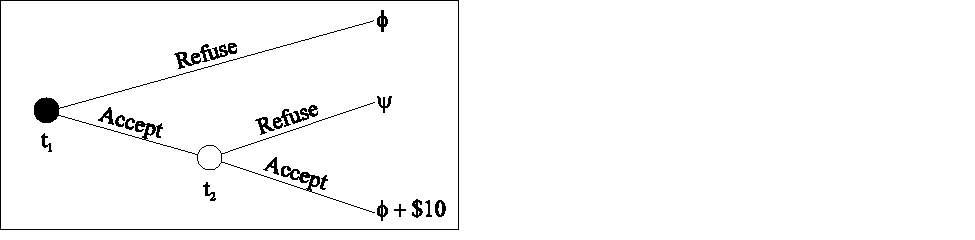
\includegraphics{vdt_tree.pdf}

}

\caption{Figure 1}

\end{figure}%

Here's what goes wrong with this objection. When considering the first
swap, the Conservative won't be comparing ψ and ϕ; rather they will be
comparing holding ψ with the possibility of having a choice between
having ϕ and having ψ~+~\$10. If they had the latter choice, they would
choose ψ~+~\$10, hence the original choice is between ψ and ψ +~\$10.
That isn't much of a choice at all, they will clearly choose the
ψ~+~\$10. That is, it is consistent with the Conservative rule to accept
both trades.

So this objection fails because it relied on a too simplistic
Conservative rule. However, a similar objection can succeed. Alter the
payout of accepting both trades to ψ +~\$5, and assume this is strictly
preferred to ψ, but almost indifferent to ϕ. Now the initial choice is a
choice between holding on to ψ, and having the choice between holding ϕ
or trading it for ψ~+~\$5. The Conservative knows if they have that
choice they will hold onto ϕ. So now the initial choice reduces to a
choice between holding ψ and trading it for ϕ. Again, the Conservative
here prefers to hold ψ. But this is absurd. Whatever we should end up
with in this circumstance, it isn't ψ, as there is some other option
strictly preferred to it. It might be noted that the use of
decision-trees in this argument, as opposed to the flawed argument given
above, is entirely standard.

There are two ways out of this problem for the Conservative, neither of
them particularly attractive. The first is to make the move Levi makes
above, to say that an agent should adopt a strategy for getting through
a decision-tree and refuse to reconsider it at later stages. The above
objections to that move still apply. The other move is to deny the
following rule for reducing complex bets to simple bets.

\begin{quote}
\emph{Reduction}: If C(β,~χ)~=~δ for any δ~∈~\{β,~χ\}, then
C(α,~(β,~χ))~=~C(α,~δ).
\end{quote}

To explain the notation, by C(α,~β)~=~α I mean that in a choice between
holding α and trading it for β, it is rationally compelling that α be
chosen. The underlining on α indicates that α is what is currently held;
this is important because by the Conservative's lights C(α,~β)~=~α and
C(α,~β)~=~β is consistent. C(α,~(β,~χ))~=~δ (δ~∈~\{α,~β,~χ\}) means that
an agent facing the choice between holding α and trading it for β with
the knowledge that this can in turn be traded for χ will end up holding
δ. Note that I don't assume C(α,~β)~is always defined.

I don't have any particularly strong arguments for \emph{Reduction}, but
it does have a high degree of intuitive plausibility. It is hard to see
what other approach could be taken. If anyone thinks it is possible to
justify avoiding \emph{Reduction} and hence can avoid this problem I
might not have much of a reply. I don't know of any such justification,
and I can't see how it could be intuitively plausible, but I'm not going
to try and write knock-down objections to as yet unformulated
justifications.\footnote{Seidenfeld
  (\citeproc{ref-Seidenfeld1994}{1994}) rejects the idea that C(α, (β,
  χ)) = C(α, β, χ), i.e.~the idea that the dynamic choice can be reduced
  to a three way static choice. He thinks it is plausible that C(α, (β,
  χ)) = α even when β has a higher payout than α on every possible state
  of affairs. But nevertheless he accepts, at page 459n,
  \emph{Reduction}, which he calls `backward induction', showing that
  the attractiveness of this principle is to a large extent independent
  of one's views on related principles concerning dynamic and static
  decisions, or equivalently concerning extensional and normal form
  decisions.}

\section{Caprice}\label{caprice}

To set out the correct decision-rule, Caprice, I need a new piece of
terminology. Say ϕ is \emph{almost preferred} to ψ according to P iff
for all \emph{Pr} in \emph{P},
\emph{E\textsubscript{Pr}}(ϕ)~≥~\emph{E\textsubscript{Pr}}(ψ). When no
ambiguity results I omit the 'according to P. Clearly whenever ϕ is
strictly preferred to ψ it is almost preferred, but the converse is not
true. Unlike strict preference, almost preference is not anti-symmetric.
Bets ϕ and ψ can each be almost preferred to the other.

The core idea behind Caprice is that there should be as few restrictions
on rational choice as possible apart from the rule that, whenever ϕ is
strictly preferred to ψ it is irrational to choose ψ over ϕ.
Unfortunately, as it is, this won't do, because it permits the following
irrational course of action. Recall the earlier example where ψ and ϕ
are almost indifferent, as are ψ~+~\$5 and ϕ. If there were no rational
restrictions on trade between almost indifferent bets then there would
be no grounds for criticising the trader who first swaps ψ~+~\$5 for ϕ
and then swaps ϕ for ψ. Yet presumably it should be possible to subject
this person to rational criticism.

I think the best thing to say about this case is that neither trade is
itself irrational, but they are an irrational combination. In most
decision-theories on the market this option is ruled out by stipulation;
a set of trades is irrational iff one member of that set is irrational.
There is, however, no reason to make such a restriction. Consider this
analogy with belief. It seems plausible to say that it is reasonable to
believe Oswald killed Kennedy and reasonable to believe he didn't, but
it isn't reasonable to believe both that Oswald killed Kennedy and that
he didn't. A set of beliefs, each reasonable on its own, might be
unreasonable in combination. I claim we can say the same about
decisions. A set of decisions, each reasonable on its own, might be
unreasonable.

Because of this intuition, the Caprice rule must be expressed in terms
of the reasonableness of sets of decisions. This can be applied easily
to simple choices by looking at singleton sets. The notation
\#(α,~β)~=~δ (δ~∈~\{α,~β\}) means that δ is chosen (by the agent under
consideration) in a pairwise choice between α and β. This is a different
concept to the earlier C(α,~β) notation in two respects. First, it is
descriptive not normative. Given that I am usually discussing ideal
agents this isn't as big a difference as it might normally seem.
Secondly, \#(α,~β) can be defined, even for rational agents, when
C(α,~β) is not. If α and β are almost indifferent, but when faced with
the choice between them the agent chooses α, then C(α,~β) is undefined
(according to Caprice), but \#(α,~β)~=~α.

\begin{quote}
\emph{Caprice}: A set \emph{S} of choices of the form
\#(α\textsubscript{i},~β\textsubscript{i})~=~α\textsubscript{i}
(i~∈~\{1,~\ldots, \emph{n},~\ldots\}) is rationally permissible
according to P iff there is some non-empty subset G of P such that for
all i, α\textsubscript{i} is almost preferred to β\textsubscript{i}
according to G .
\end{quote}

Caprice is only defined in terms of pairwise choices. If α is chosen in
a three-way choice between α, β and χ, we say \#(α,~β)~=~α and
\#(α,~χ)~=~α. This can easily be extended to \emph{n}-way choices. Hence
a single \emph{n}-way choice, with \emph{n}~\textgreater~2, can be
regarded as a many-element set of pairwise choices.

Note two immediate consequences of this rule. First, when we are just
considering a single choice between almost indifferent bets ψ and ϕ,
either choice is acceptable. In trading terms, it is permissible but not
compelling to trade ψ for ϕ. This is the motivation for calling the rule
`Caprice'. Secondly, any set of choices which leaves the trader with a
position such that they would strictly prefer to be back where they
started is not rationally permissible according to Caprice. Hence
Caprice as specified captures two important intuitive requirements on
decision-rules.

I haven't yet specified how Caprice should be applied to choices between
nodes of a decision-tree, because here there isn't much to say. In cases
like that set out in Figure 1, the Capricious decision-maker can simply
decide which end-point she wants to end up with, and follow the tree to
that point. Provided her original \emph{n}-way choice is permissible,
every pair-wise choice she makes will be permissible. I showed above
that the only way for the Conservative to avoid absurd decisions was to
be closed-minded in the sense that she had to deliberately decide
\emph{not} to reflect at various stages in the tree about whether her
initial strategy should be carried through. By comparison, the
Capricious agent can be completely reflective.

There is one interesting special case of Caprice, which I'm adopting
from Smets (\citeproc{ref-Smets1994}{1994}). It isn't Smets's preferred
approach for a couple of reasons, not least being that Smets advocates
dropping conditionalisation, but the terminology and idea is largely
his. An agent whose representor is P has P as their \emph{credal}
probability function. They arbitrarily select an element \emph{Pi} from
P to use for decision-making purposes; this is their \emph{pignistic}
probability. (`Pignistic' is from the Latin \emph{pignus}, meaning to
bet.) When making a choice between gambles they choose that gamble α
such that \emph{E\textsubscript{Pi}}(α) is maximised. An agent who does
this will never do anything wrong according to Caprice.

I noted at page 6 that any decision-rule would have to give up one of
Arrow's constraints (1) through (4). Caprice gives up (2). It says that
sometimes given the composition of P we simply can't say which of two
bets should be chosen. If this pignistic approach is followed, in a
sense (2) is kept at the cost of (3). The pignistic probability function
becomes the dictator in Arrow's sense. This might be an improvement; I
leave it up to the reader to decide whether or not it is.

There is one odd result as a consequence of adopting Caprice. An agent
is told (reliably) that there are red and black marbles in a box in
front of them, and a marble is to be drawn from the box. They are given
the choice between three bets. α pays \$1 if a red marble is drawn,
nothing otherwise, β pays a certain 45 cents, and χ pays \$1 if a black
marble is drawn. Is it rationally permissible for the agent to choose β,
again assuming constant marginal utility of money?

Levi (\citeproc{ref-Levi1974}{1974}) writes as if it is obvious that
choosing β is irrational. This is a cornerstone of the `impeccable'
analysis which leads to a dismissal of (4) but receives almost no
justification. Jeffrey (\citeproc{ref-Jeffrey1983}{1983}) defines
Bayesian approaches to decision-making so that choosing β is not
Bayesian, but of course it isn't an obvious truth that only Bayesian
approaches are correct. Dempster (\citeproc{ref-Dempster1988}{1988})
claims that choosing β is permissible, and perhaps even compelling,
though it appears he is motivated by the maximin rule, which I showed
above is flawed.

I only bring this up to note that Caprice says it is not rational to
choose β. To see this, assume we choose β. We will now show that G must
be empty. Let \emph{p} be the proposition that the marble to be drawn is
red. Since β is almost preferred to α according to G , for every
\emph{Pr} in G it follows that \emph{Pr}(\emph{p})~≤~0.45. However,
since β is almost preferred to χ according to G , for every \emph{Pr} in
G it follows that \emph{Pr}(\emph{p})~≥~0.55. There is no \emph{Pr}
satisfying each of these constraints, hence G is empty. It doesn't
however, appear at all intuitively compelling that it should be
irrational to choose β. A defender of Caprice has to either explain away
this intuition or, like Levi, simply deny that the intuition exists. The
first of these choices is possible. One approach already noted is to say
a choice of β reflects an irrational commitment to Maximin. Another is
to say that it reflects a failure to internalise fully the assumption
that the marginal utility of money is constant. I suspect that is what
explains my intuition that β is an acceptable choice. I don't think this
raises a huge problem for the defender of Caprice -- some questions are
always going to be spoils to the victor -- but it is a little
disconcerting. If there is to be a strong attack on Caprice, I suspect
it will be built around cases like this one.

\section{Arguments For Caprice}\label{arguments-for-caprice}

Apart from the fact that it avoids the pitfalls of its more well-known
rivals, there are two positive arguments for Caprice. Each of them is
essentially the reverse of an argument I used against Levi. I'll call
them the arguments from Arrow and Buridan.

The argument from Arrow notes that the four principles Arrow gave, (1)
to (4) above, are inconsistent. Hence we must give up one of them. As
there is strong intuitive support for Pareto, Non-Dictatorship and
Independence of Irrelevant Alternatives, it seems the correct decision
theory must give up what Arrow calls `Collective Rationality', but what
is perhaps better called Completeness in our context. There must be some
choices about which our decision theory is silent. Since Caprice, unlike
its popular rivals, satisfies this constraint, this is something in its
favour. Of course this is not an argument against other incomplete
rivals of Caprice. However, one strength of Caprice is that the class of
decisions over which it is silent is quite a natural class. I doubt
there could be a smaller class than this which is equally natural.

This leads to the argument from Buridan. Given the way I have set out
the problem, when ψ and ϕ are almost indifferent, there is no reason to
choose one over the other. The agent really is in the position of
Buridan's ass. Of course like the ass the agent may be well advised to
choose either ψ or ϕ over some less attractive alternatives. Unlike all
its rivals, Caprice takes this conclusion seriously. If there is no
reason to choose ψ over ϕ or \emph{vice versa}, there really is no
reason. It doesn't go and say this and then find a reason.

In particular, it must be really inexplicable why an agent chooses ψ
over ϕ or \emph{vice versa} in such cases. Should there be such a
reason, it must be traceable to the beliefs and desires (or more
generally partial beliefs and preferences) of the agent. The assumption
of incomparability is just the assumption that those beliefs and desires
don't determine a choice. Hence any decision theory must agree with
Caprice's `no explanation' conclusion. Given this, it is hard to see how
the correct theory can differ from Caprice.

It might be thought that Caprice breaches this `no explanation' rule in
an important case. Say the expected value of ψ is vague over {[}\$30,
\$40{]}, and that an agent has just sold a unit of ψ for \$32. According
to Caprice, if she now buys a unit for \$38, or indeed any price over
\$32, she will have acted irrationally. Does this mean that either (i)
the value of ψ is now vague over merely {[}\$30, \$32{]} or (ii) the
value is unchanged but she now has a reason for not buying ψ for more
than \$32? According to the objection, I have ruled out (i) and (ii),
but I am committed to one of them.

The objection is in part correct, I have ruled out (i) and (ii).
However, I am not committed to their disjunction. Were the agent to now
buy ψ for \$38, that would not of itself be an irrational act, however
it would take her from having performed a set of rational acts to having
performed a set of irrational ones. The only reason one would think this
implies the last act is irrational is if one was wedded to the idea that
a set of acts is irrational iff it includes an irrational act. By that
principle, an agent can only move from a rational to an irrational set
by performing an irrational act. However, that is a principle I gave
reasons for rejecting in setting out Caprice.

Again the analogy with belief is instructive. If the agent believed
yesterday that Oswald killed Kennedy, she can't rationally believe today
that Oswald didn't kill Kennedy unless she ceases to believe that he did
kill him. But, and here's the difference, yesterday's beliefs can be
more easily undone than yesterday's trades. If she could cease to have
sold ψ for \$32 yesterday, she can rationally buy it for \$38 today.
Sometimes this will be possible (if the sale has a `cooling off'
period), but usually it will be just as fixed as the rest of the past.
It is because she can change her beliefs, but not her trades, that we
judge an agent's trades diachronically, but her beliefs largely
synchronically. When we keep all this in mind, we won't unduly focus on
her last trade and judge it too harshly.

\section{Summary}\label{summary}

Most of the attempts to formulate a vague decision theory have been
attempts to say what ought be done when faced with almost indifferent
options. The decision theory here says that we cannot consistently
answer this question. For one thing, it is incoherent to say the options
are almost indifferent and on the other hand that we can decide between
them. This is just an admission that we have not included all the
relevant material in our representation of the agent's beliefs and
desires. Secondly, the attempts to answer the question so far have all
led to dynamic incoherence, and Arrow's Theorem suggests this is
unavoidable. So it is best to settle for the minimal constraints
supplied by Caprice.

\subsection*{References}\label{references}
\addcontentsline{toc}{subsection}{References}

\phantomsection\label{refs}
\begin{CSLReferences}{1}{0}
\bibitem[\citeproctext]{ref-Arrow1963}
Arrow, Kenneth J. 1963. \emph{Social Choice and Individual Values}. New
York: Wiley.

\bibitem[\citeproctext]{ref-Dempster1988}
Dempster, Arthur. 1988. {``Probability, Evidence and Judgment.''} In
\emph{Decision Making}, edited by D. Bell, H. Raiffa, and A. Tversky,
283--98. Cambridge University Press.

\bibitem[\citeproctext]{ref-vanFraassen1990}
Fraassen, Bas van. 1990. {``Figures in a Probability Landscape.''} In
\emph{Truth or Consequences}, edited by J. M. Dunn and A. Gupta,
345--56. Amsterdam: Kluwer.

\bibitem[\citeproctext]{ref-vanFraassen1995}
---------. 1995. {``Belief and the Problem of Ulysses and the Sirens.''}
\emph{Philosophical Studies} 77 (1): 7--37. doi:
\href{https://doi.org/10.1007/bf00996309}{10.1007/bf00996309}.

\bibitem[\citeproctext]{ref-GilboaSchmeidler1993}
Gilboa, Itzhak, and David Schmeidler. 1993. {``Updating Ambiguous
Beliefs.''} \emph{Journal of Economic Theory} 59 (1): 33--49. doi:
\href{https://doi.org/10.1006/jeth.1993.1003}{10.1006/jeth.1993.1003}.

\bibitem[\citeproctext]{ref-Hajek2000}
Hájek, Alan. 2000. {``Objecting Vaguely to Pascal's Wager.''}
\emph{Philosophical Studies} 98: 1--16. doi:
\href{https://doi.org/10.1023/A:1018329005240}{10.1023/A:1018329005240}.

\bibitem[\citeproctext]{ref-Hart1942}
Hart, A. G. 1942. {``Risk, Uncertainty and the Unprofitability of
Compounding Probabilities.''} In \emph{Studies in Mathematical Economics
and Econometrics}, edited by F. McIntyre O. Lange and T. O. Yntema.,
110--18. Chicago: University of Chicago Press.

\bibitem[\citeproctext]{ref-Hausman1991}
Hausman, Daniel. 1991. \emph{The Inexact and Separate Science of
Economics}. Cambridge: Cambridge University Press.

\bibitem[\citeproctext]{ref-Jaffray1994}
Jaffray, J. Y. 1994. {``Decision Making with Belief Functions.''} In
\emph{Advances in the Dempster- Shafer Theory of Evidence}, edited by R.
Yager, M. Fedrizzi, and J. Kacprzyk, 331--52. New York: John Wiley.

\bibitem[\citeproctext]{ref-Jeffrey1983}
Jeffrey, Richard. 1983. {``Bayesianism with a Human Face.''} In
\emph{Testing Scientific Theories}, edited by J. Earman (ed.).
Minneapolis: University of Minnesota Press.

\bibitem[\citeproctext]{ref-Levi1974}
Levi, Isaac. 1974. {``On Indeterminate Probabilities.''} \emph{Journal
of Philosophy} 71 (13): 391--418. doi:
\href{https://doi.org/10.2307/2025161}{10.2307/2025161}.

\bibitem[\citeproctext]{ref-Levi1980}
---------. 1980. \emph{The Enterprise of Knowledge}. Cambridge, MA.: MIT
Press.

\bibitem[\citeproctext]{ref-Levi1986}
---------. 1986. \emph{Hard Choices}. Cambridge: Cambridge University
Press.

\bibitem[\citeproctext]{ref-Levi1987}
---------. 1987. {``The Demons of Decision.''} \emph{Monist} 70 (2):
193--211. doi:
\href{https://doi.org/10.5840/monist198770215}{10.5840/monist198770215}.

\bibitem[\citeproctext]{ref-Norton1998}
Norton, John. 1998. {``When the Sum of Our Expectations Fails Us.''}
\emph{Pacific Philosophical Quarterly} 79 (1): 34--58. doi:
\href{https://doi.org/10.1111/1468-0114.00049}{10.1111/1468-0114.00049}.

\bibitem[\citeproctext]{ref-RamseyTruthProb}
Ramsey, Frank. 1926. {``Truth and Probability.''} In \emph{Philosophical
Papers}, edited by D. H. Mellor, 52--94. Cambridge: Cambridge University
Press.

\bibitem[\citeproctext]{ref-Seidenfeld1984}
Seidenfeld, Teddy. 1984. {``Review of Paul Horwich, \emph{Probability
and Evidence}.''} \emph{Philosophical Review} 93 (3): 474--83. doi:
\href{https://doi.org/10.2307/2184556}{10.2307/2184556}.

\bibitem[\citeproctext]{ref-Seidenfeld1994}
---------. 1994. {``When Normal and Extensive Form Decisions Differ.''}
In \emph{Logic, Methodology and Philosophy of Science}, edited by Brian
Skyrms Dag Prawitz and Dag Westerståhl, 451--63. Amsterdam: Elsevier.

\bibitem[\citeproctext]{ref-Smets1994}
Smets, Philippe. 1994. {``What Is Dempster-Shafer's Theory of
Evidence?''} In \emph{Advances in the Dempster-Shafer Theory of
Evidence}, edited by Yager, Fedrizzi, and Kacpzyk, 5--34. Wiley.

\bibitem[\citeproctext]{ref-Smith1961}
Smith, Cedric A. B. 1961. {``Consistency in Statistical Inference and
Decision.''} \emph{Journal of the Royal Statistical Society Series B}
23: 1--37.

\bibitem[\citeproctext]{ref-Strat1990}
Strat, Thomas. 1990. {``Decision Analysis Using Belief Functions.''}
\emph{International Journal of Approximative Reasoning} 4 (5-6):
391--417. doi:
\href{https://doi.org/10.1016/0888-613x(90)90014-s}{10.1016/0888-613x(90)90014-s}.

\bibitem[\citeproctext]{ref-Tintner1941}
Tintner, Gerhard. 1941. {``The Theory of Choice Under Subjective Risk
and Uncertainty.''} \emph{Econometrica} 9 (3/4): 298--304. doi:
\href{https://doi.org/10.2307/1907198}{10.2307/1907198}.

\bibitem[\citeproctext]{ref-Walley1991}
Walley, Peter. 1991. \emph{Statisical Reasoning with Imprecise
Probabilities}. London: Chapman \& Hall.

\bibitem[\citeproctext]{ref-Williams1976}
Williams, Peter. 1976. {``Indeterminate Probabilities.''} In
\emph{Formal Methods in the Methodology of the Empriccal Sciences},
edited by M. Przelecki, K. Szaniawski, and R. Wojcicki, 229--46.
Dordrecht: Reidel.

\bibitem[\citeproctext]{ref-Williams1978}
---------. 1978. {``On a New Theory of Epistemic Probability.''}
\emph{British Journal for the Philosophy of Science} 29 (4): 375--87.
doi:
\href{https://doi.org/10.1093/bjps/29.4.375}{10.1093/bjps/29.4.375}.

\end{CSLReferences}



\noindent Unpublished. Draft of October 1998.

\end{document}
